\section{RECOVERY}

\subsection{Airfield}

The standard VFR recovery for 108\th will be the Overhead Break, subject to
Tower permission. Coming from a 2-5NM Initial (check charts, if available), the
standard Run-In into the Overhead is performed with 300 KCAS and wings 68°
fully aft \textbf{MAN}ual

\sidebyside{0.6}{%

  Altitude for the OHB is set by local airfield noise abatement procedures and
  geographical restrictions which are usually published in charts under
  'Closed Pattern Altitude'.

  With no other constraints, it shall be 1500 feet above field elevation,
  in echelon, away from the tower, populated areas, or other runways, or to the
  left, with sufficient intervals for a safe arrival:

  \begin{itemize}
    \item Formation in-trail with a handfull of hundreds feet inbetween each
      for a common full-stop landing, this may be in the region of 2-5 second
      intervals.

    \item If you wish to split the formation into individual single-ships with
      different individual intentions such as follow-up pattern training a
      larger spacing of 10-20 sec intervals are required to enable safe
      separation between a touch-and-go behind a full-stop.
    \end{itemize}

  Please refer to the \href
    {https://cloud.132virtualwing.org/s/ga9qYFdSDeGN7dy}
    {132\nd TTP-5 ATC Airbase Operations}
  for further information regarding wing wide policies.

}{%
  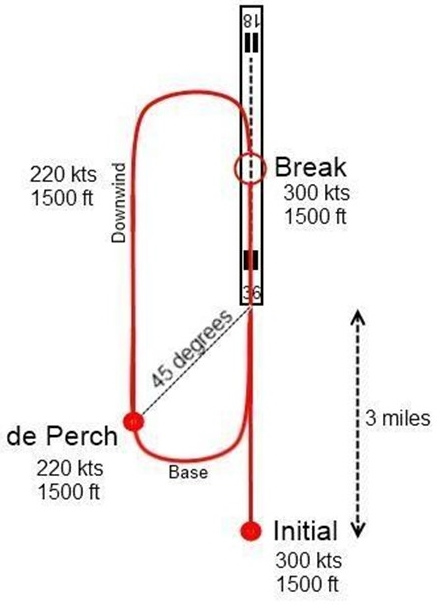
\includegraphics[width=\textwidth,align=t]{recovery/airfield}
}

Minimum spacing between sequentially landing aircraft is 3000 feet (0.5 nm), or
6000 feet (1 nm) with high wind or turbulence. Wake turbulence is currently
something to watch out for in tight sequences and the actual minimums could be
revised.

Formation approaches are not permitted under the following conditions:

\begin{itemize}
  \item There is a crosswind component exceeding 15 kts
  \item The runway is wet or slippery
  \item The runway width is < 125 feet
  \item The weather has a ceiling lower than 500 feet AGL
  \item Asymmetric stores loadouts
  \item Unsafe loadouts like hung ordnance
\end{itemize}

\subsection{Carrier}

Please review \href
  {https://cloud.132virtualwing.org/s/wSMBb66EEEJztNW}
  {132\nd TTP-19 Carrier Operations}
